
为了找到一个对性能的关注从未减弱的例子,让我们来看看计算的演变(它使计算本身成为可能),\textbf{电子设计自动化(EDA)}工具,其会用来设计计算机。

在2010年进行了设计、模拟或验证某一特定微芯片的计算,此后每年都运行相同的计算量,我们会看到这样的结果:

%\hspace*{\fill} \\ %插入空行
\begin{center}
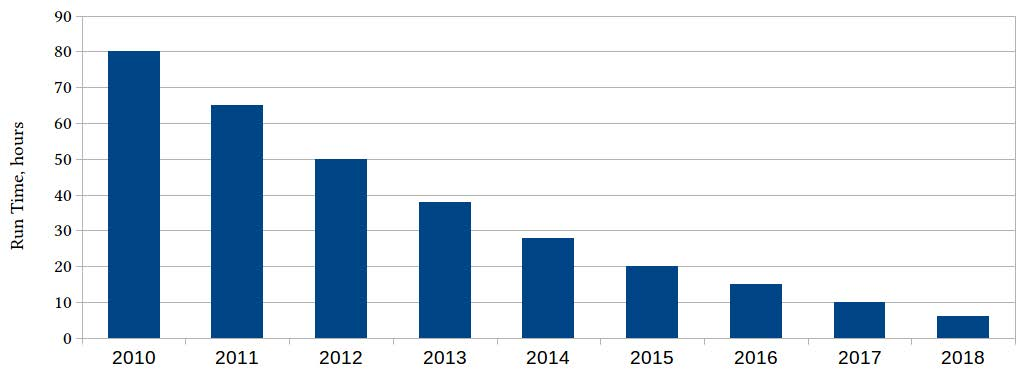
\includegraphics[width=0.9\textwidth]{content/1/chapter1/images/2.jpg}\\
图1.2 - 这些年来对于特定的EDA计算的处理时间,以小时为单位,
\end{center}

2010年计算时间为80小时,而2018年计算时间不到10小时(现在更短)。改善从何而来?计算机变得更快,但同时软件变得更高效,使用更好的算法,优化的编译器变得更有效。

当然,我们不会在2021年制造2010版的微芯片:有理由认为,随着电脑变得越来越强大,制造更新更好的芯片变得越来越困难。那么,更有趣的问题是,我们每年要花多长时间才能完成同样的工作呢?

%\hspace*{\fill} \\ %插入空行
\begin{center}
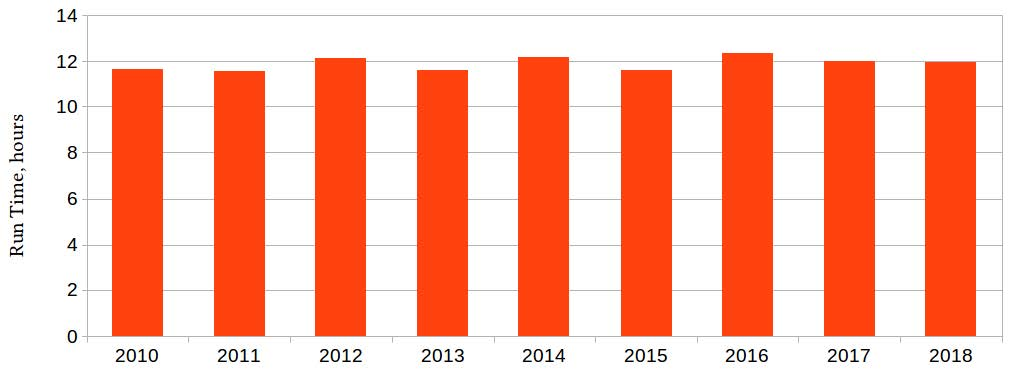
\includegraphics[width=0.9\textwidth]{content/1/chapter1/images/3.jpg}\\
图1.3 - 每年最新的微芯片的运行时间,以小时为单位
\end{center}

每年实际完成的计算并不相同,但它们的目的是相同的,例如:验证芯片是否按照预期的方式运行,对于我们每年制作的芯片。从这个图表可以看出,当前最强大的处理器,运行可用的最佳工具时,每年设计和建模下一代处理器所用的时间大致相同。虽然我们还在努力,但没有任何进展。

事实比这更糟,上面的图表并不能说明一切。从2010年到2018年,那一年生产的最大处理器可以在一夜之间(大约12个小时)通过适配去年生产的电脑进行验证。这里,我们忘了问有多少个处理器?好吧,下面就是真相:

%\hspace*{\fill} \\ %插入空行
\begin{center}
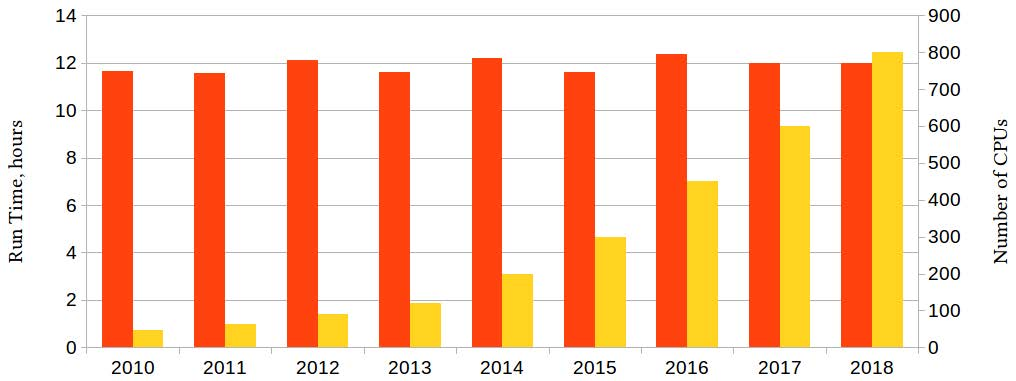
\includegraphics[width=0.9\textwidth]{content/1/chapter1/images/4.jpg}\\
图1.4 - 添加了每次计算的CPU数量
\end{center}

每年好的计算机,配备了数量不断增长的处理器,运行最新的软件版本(优化会利用越来越多的处理器,并更有效地使用每个处理器),完成构造下一年计算机所需的工作,每年都是在这样,但这项任务几乎不可能完成。我们依靠硬件和软件工程师的成就而保持一优势,因为前者提供了不断增长的计算能力,而后者则以最高的效率使用它。这本书将来了解后者所使用的技能。

我们现在明白了这本书中内容的重要性。在深入研究细节之前,做一个高层概述可能会有所帮助。


















